\documentclass[11pt,twoside]{estiloUBI}

%%%%%%%%%%%%%%%%%%%%%%%%%%%%%%%%%%%%%%%%%%%%%%%%%%%%%%%%%%%%%%%%%%%%%%%%%%%%%%%%%%%%%%%%%%%%%%%%%%%%%%%%%%%%%%
%% Este é o ficheiro formatacaoUBI.tex - NÃO EDITAR excepto a secção hypersetup!
%% Define a formatação a ser usada em teses apresentadadas na Universidade da Beira Interior, seguindo o despacho Reitoral nº 49/R/2010
%% Versão 2.2 - 01/06/2016 - Podem aparecer as palavras "Figura" e "Tabela" nas respectivas listas
%% Versão 2.1 - 28/03/2014 - Agora compila com o XeLaTeX por causa do tipo de fonte, incluido o estilo de biblipgrafia IEEE, possibilidade de escolha de tipo de fonte matemático
%% Versão 2.0 - 10/11/2011 - Bibliografia agora aparece no índice
%% Versão 1.9 - 10/10/2011 - Resolvido problema em que o texto nas tabelas aparecia em cima da linha superior
%% Versão 1.8 - 12/07/2011 - Legendas são agora centradas
%% Versão 1.7 - 8/07/2011 - Correcção de algumas medidas de acordo com novo modelo de Word
%% Versão 1.6 - 1/07/2011 - Trebuchet inserido como fonte principal
%% Adaptado do original de Oliver Commowick para estar de acordo com as regras do Despacho nº 49/R/2010
%% Adaptação por João Ferro, Norberto Barroca, Luís Borges, Rui Paulo, Aleksandra Nadziejko - Instituto de Telecomunicações - DEM/UBI, Paulo Machado - Departamento de Ciências Aeroespaciais/UBI.
%% Contacto: latex@e-projects.ubi.pt
%% Agradecimento especial a Stefan_K da latex-community.org pela ajuda com os códigos de tabela e equação.
%% A versão actual pode ser alterada sem aviso prévio.
%% Download da última versão em área reservada: http://www.UBI.pt
%% Uso e distribuição de acordo com a licenca GNU GPL.
%% 
%%    Este programa é um software livre: você pode redistribui-lo e/ou 
%%
%%		modificá-lo dentro dos termos da Licença Pública Geral GNU como 
%%
%%		publicada pela Free Software Foundation, na versão 3 da 
%%
%%		Licença, ou (na sua opinião) qualquer versão.
%%
%%
%%
%%		Este programa é distribuido na esperança que possa ser útil, 
%%
%%		mas SEM NENHUMA GARANTIA; sem uma garantia implícita de ADEQUAÇÃO a qualquer
%%
%%		MERCADO ou APLICAÇÃO EM PARTICULAR. Veja a
%%
%%		Licença Pública Geral GNU para maiores detalhes.
%%
%%
%%
%%		Você deve ter recebido uma cópia da Licença Pública Geral GNU
%%
%%		junto com este programa, se não, veja <http://www.gnu.org/licenses/>.
%%%%%%%%%%%%%%%%%%%%%%%%%%%%%%%%%%%%%%%%%%%%%%%%%%%%%%%%%%%%%%%%%%%%%%%%%%%%%%%%%%%%%%%%%%%%%%%%%%%%%%%%%%%%%%


% Pacotes a incluir
\usepackage{mathspec}
\usepackage{fontspec}
\usepackage{amsmath,amscd,amsthm,xspace}	%Pacotes matemáticos 
\usepackage{amssymb}						%Fontes extra para matemáticos   http://www.ctan.org/tex-archive/fonts/amsfonts
%\usepackage[math]{kurier} %descomentar para colocar tipo de letra aproximado ao Trebuchet nos ambientes matemáticos

%\usepackage[latin1]{inputenc}		%este faz falta na versão normal, mas em XeLaTeX tem que ser comentado		%Permitir caracteres acentuados  http://www.ctan.org/pkg/inputenc
%\usepackage[T1]{fontenc}					%este faz falta na versão normal, mas em XeLaTeX tem que ser comentado		%Permitir caracteresespeciais  http://www.ctan.org/pkg/fontenc

\usepackage[a4paper,left=3.5cm,right=2.5cm,top=2.5cm,bottom=2.5cm]{geometry}	%Papel A4, com margens
%\renewcommand{\baselinestretch}{1.05}

\usepackage{aecompl}								%Permitir fontes vituais para codificação T1  http://www.ctan.org/tex-archive/fonts/ae
\usepackage[center,nooneline,font={footnotesize}]{caption}			%Legenda: centrada, tamanho de nota rodapé  http://www.ctan.org/pkg/caption
\setlength{\parindent}{0pt}							%Sem tabulação em cada novo parágrafo
%\usepackage{parskip}								%Layout with zero \parindent, non-zero \parskip http://www.ctan.org/pkg/parskip
%\setlength{\parskip}{0.53cm}



%% O código seguinte permite gerar um mini indice de capitulo (não referido no despacho reitoral)
% \usepackage[nottoc, notlof, notlot]{tocbibind}
% \usepackage{minitoc}
% \setcounter{minitocdepth}{2}
% \mtcindent=15pt
%%Usar \minitoc para colocar o mini indice de capitulo


%% Verificar se saída é pdf directo e ajustar o formato imagens a isso
%\usepackage{ifpdf}
%\ifpdf
%  \usepackage[pdftex]{graphicx}							%Inserir gráficos  http://ctan.org/pkg/graphicx
\usepackage{graphicx}
%    \DeclareGraphicsExtensions{.jpg,.png} 					%Pdf directo apenas compativel com jpg, png...
  \usepackage[pagebackref,hyperindex=true]{hyperref}				%O pacote hyperref é usada para lidar com comandos referência cruzada  http://ctan.org/pkg/hyperref
%\else
%  \usepackage{graphicx}
%  \DeclareGraphicsExtensions{.ps,.eps}						%DVI directo apenas compativel com ps, eps...
%  \usepackage[dvipdfm,pagebackref,hyperindex=true]{hyperref}
%\fi


\graphicspath{{.}{imagens/}}							%Directorio das imagens


%%Links do pdf
\usepackage{color}								%Pacote de gestão de cor
\definecolor{linkcol}{rgb}{0,0,0} 						%Cor das hiperligações (preto)
\definecolor{citecol}{rgb}{0,0,0} 						%Cor das referências à bibliografia no texto (preto)


%% O código seguinte será incluído no pdf gerado http://www.tug.org/applications/hyperref/manual.html
%%Visto nas propriedades do documento
% \hypersetup
% {
% bookmarksopen=true,
% pdftitle="Tese",		%Título
% pdfauthor="João", 		%Autor
% pdfsubject="Tese", 		%Assunto
% pdfmenubar=true,		%Mostrar barra menus
% pdfhighlight=/O, 		%Efeito ao clicar link
% colorlinks=true, 		%Cor em hiperligações
% pdfpagemode=UseNone, 		%Nenhum modo de páginas
% pdfpagelayout=SinglePage, 	%Abertura em modo de página simples
% pdffitwindow=true, 		%Adaptar página à janela
% linkcolor=linkcol, 		%Cor das ligações internas do documento
% citecolor=citecol, 		%Cor das referências à bibliografia no texto
% urlcolor=linkcol 		%Cor das hiperligações
% }


%%Definições variadas
\setcounter{secnumdepth}{3}
\setcounter{tocdepth}{2}


%%Comandos e atalhos para algumas funções matemáticas
\newcommand{\pd}[2]{\frac{\partial #1}{\partial #2}}
\def\abs{\operatorname{abs}}
\def\argmax{\operatornamewithlimits{arg\,max}}
\def\argmin{\operatornamewithlimits{arg\,min}}
\def\diag{\operatorname{Diag}}
\newcommand{\eqRef}[1]{(\ref{#1})}


%%Para rotação de figuras e tabelas http://www.ctan.org/tex-archive/macros/latex/contrib/rotating
 \usepackage{rotating}
  
	
%%Cabeçalho e rodapé http://www.ctan.org/tex-archive/macros/latex/contrib/fancyhdr
\usepackage{fancyhdr}                   						%Fancy Header and Footer
\pagestyle{fancy}                      							%Cabeçalho e rodapé estilo fancy
\fancyfoot{}                            						%Apaga rodapé actual
\fancyhead{}										%Apaga cabeçalho actual
\fancyfoot[LE,RO]{\thepage}   								%Número de paginas no exterior L=left, E=even, R=right, O=Odd
\newcommand{\cabecalho}[1]{\fancyhead[RE,LO]{\bfseries{#1}}}				%Nome da tese no cabeçalho
\let\headruleORIG\headrule
\renewcommand{\headrule}{\color{black} \headruleORIG}
\renewcommand{\headrulewidth}{0pt}							%Régua para cabecalho, 0pt=off, 1pt=on


%Formatação dos tipos de letra
\newcommand{\capitulos}{\fontsize{22pt}{10pt}\bfseries\selectfont}			%Capítulo: 22pt, negrito
\newcommand{\titulos}{\fontsize{18pt}{10pt}\bfseries\selectfont}			%Titulos: 18pt, negrito
\newcommand{\seccao}{\fontsize{14pt}{20pt}\bfseries\selectfont}				%Secção: 14pt, negrito
\newcommand{\subseccao}{\fontsize{12pt}{14pt}\selectfont}				%subsecção: 12pt, normal
\renewcommand{\footnotesize}{\fontsize{9pt}{12pt}\selectfont}				%Nota rodapé: 9pt, espacamento 1 linha
\renewcommand{\Huge}{\titulos}


%Folha de rosto
\newcommand{\rostoubi}{\fontsize{14pt}{14pt}\selectfont}				%Texto a dizer UBI 14pt, normal
\newcommand{\rostotitulo}{\fontsize{18pt}{18pt}\selectfont}				%Titulo da tese: 18pt, (+negrito)
\newcommand{\rostosubtit}{\fontsize{16pt}{16pt}\selectfont}				%Titulo da tese: 16pt, (+negrito)
\newcommand{\rostonomes}{\fontsize{14pt}{14pt}\selectfont}				%Nome autor, curso: 14pt, (+negrito)
\newcommand{\rostooutros}{\fontsize{12pt}{12pt}\selectfont}				%Local e data: 12pt, (+negrito)
\newcommand{\rostofac}{\fontsize{12.5pt}{12.5pt}\selectfont}				%Faculdade: 12.5pt




%%Passar para português
%\newcommand{\portugues}{\usepackage[portuguese]{babel}		%Descomentar para escrever com regras em Português sem ser em XeLaTeX  http://www.ctan.org/pkg/babel  								% Users of X∃TeX are ad­vised to use poly­glos­sia rather than Ba­bel.

\newcommand{\portugues}{\usepackage{polyglossia} %Comentar para escrever sem ser em modo XeLaTeX http://www.ctan.org/tex-archive/macros/latex/contrib/polyglossia
\setmainlanguage{portuges}                       %Comentar para escrever sem ser em modo XeLaTeX

\addto\captionsportuguese{\renewcommand{\contentsname}{Índice}}
\addto\captionsportuguese{\renewcommand{\indexname}{Índice Remissivo}}}

%linhas das tabelas e afins
\usepackage{colortbl}									%Adicionar cor às tabelas  http://www.ctan.org/tex-archive/macros/latex/contrib/colortbl/
\arrayrulecolor{black}									%Preto


%Estilo plain modificado
\fancypagestyle{plain}{
  %\fancyhead{}	
  %\fancyfoot{}
  \renewcommand{\headrulewidth}{0pt}
}


%%Para algoritmos  http://www.ctan.org/tex-archive/macros/latex/contrib/algorithms/
\usepackage{algorithm}
\usepackage[noend]{algorithmic}


%%Páginas em branco geradas antes de capítulos têm de vir numeradas
\makeatletter

\def\cleardoublepage{\clearpage\if@twoside \ifodd\c@page\else%
  \hbox{}%
  \thispagestyle{plain}%              							%Páginas em branco usam estilo plain
  \newpage%
  \if@twocolumn\hbox{}\newpage\fi\fi\fi}

\makeatother


%%Tabela com 9pt
%\makeatletter										%O código comentado apresentado apresenta problemas
%\renewenvironment{table}{%								%Procurar no forum http://latex-community.org, tópico "Equation Numbering and Table Font Size''
  %\@float{table}\footnotesize}
  %{\end@float}
%\makeatother
\usepackage{etoolbox}									%Para modificar o tamanho de letra na tabela http://ctan.org/pkg/etoolbox
\AtBeginEnvironment{tabular}{\footnotesize}						%Procurar no forum http://latex-community.org, tópico "Equation Numbering and Table Font Size''


%%Número de equação centrado com equação
\makeatletter										%Explicação  http://tex.stackexchange.com/questions/8351/what-do-makeatletter-and-makeatother-do
\def\place@tag{\quad\boxz@}								%Comentar esta linha para alinhar número da equação à direita
\makeatother
\let\equation\align
\let\endequation\endalign
 

%%Código herdado
\newenvironment{maxime}[1]
{
\vspace*{0cm}
\hfill
\begin{minipage}{0.5\textwidth}%
%\rule[0.5ex]{\textwidth}{0.1mm}\\%
\hrulefill $\:$ {\bf #1}\\
%\vspace*{-0.25cm}
\it 
}%
{%

\hrulefill
\vspace*{0.5cm}%
\end{minipage}
}

%mninitoc
%\let\minitocORIG\minitoc
%\renewcommand{\minitoc}{\minitocORIG \vspace{1.5em}}

\usepackage{multirow}					%Create tab­u­lar cells http://www.ctan.org/tex-archive/macros/latex/contrib/multirow
% \usepackage{slashbox}					%Pro­duce tab­u­lar cells with di­ag­o­nal lines in them http://www.ctan.org/pkg/slashbox

\newenvironment{bulletList}				%http://en.wikibooks.org/wiki/LaTeX/List_Structures
{ \begin{list}%
	{$\bullet$}%
	{\setlength{\labelwidth}{25pt}%
	 \setlength{\leftmargin}{30pt}%
	 \setlength{\itemsep}{\parsep}}}%
{ \end{list} }

\newtheorem{definition}{Définition}
\renewcommand{\epsilon}{\varepsilon}

% centered page environment

\newenvironment{vcenterpage}
%{\newpage\vspace*{\fill}\fancyhf{}\renewcommand{\headrulewidth}{0pt}}
{\newpage\vspace*{\fill}\renewcommand{\headrulewidth}{0pt}}
{\vspace*{\fill}\par\pagebreak}

\usepackage{setspace}					%Pro­vides sup­port for set­ting the spac­ing be­tween lines http://www.ctan.org/tex-archive/macros/latex/contrib/setspace
\usepackage{tabularx}					%The pack­age de­fines an en­vi­ron­ment tab­u­larx, an ex­ten­sion of tab­u­lar  http://www.ctan.org/pkg/tabularx
\usepackage{makeidx}					%Index processor  http://www.ctan.org/tex-archive/indexing/makeindex
\newcolumntype{Y}{>{\raggedright\arraybackslash}X}

%% Inicio do bloco
%% Descomentando o este bloco de comandos as  palavras "Figura" e "Tabelas" vão aparecer por extenso nas respectivas Listas
%%
%% Comentado aparece:
%%Lista de Figuras
%%		2.1 Circuito básico com uma fonte de tensão contínua (V) e uma resistência atraves-
%%			sada por uma corrente I. . . . . . . . . . . . . . . . . . . . . . . . . . . . . .3
%%
%% Descomentando aparece
%% 		Figura 2.1 Circuito básico com uma fonte de tensão contínua (V) e uma resistência
%%      atravessada por uma corrente I. . . . . . . . . . . . . . . . . . . . . .3
%%
%\usepackage[titles]{tocloft}
%\newlength{\mylen}
%
%\renewcommand{\cftfigpresnum}{\figurename\enspace}
%\renewcommand{\cftfigaftersnum}{ }
%\settowidth{\mylen}{\cftfigpresnum\cftfigaftersnum}
%\addtolength{\cftfignumwidth}{\mylen}
%
%\renewcommand{\cfttabpresnum}{\tablename\enspace}
%\renewcommand{\cfttabaftersnum}{ }
%\settowidth{\mylen}{\cfttabpresnum\cfttabaftersnum}
%\addtolength{\cfttabnumwidth}{\mylen}
%% Fim do Bloco


\usepackage{caption}

\usepackage[stable]{footmisc}

\usepackage{fontspec} 

\usepackage{polyglossia}
\usepackage{forest}

\setmainlanguage{english}

%%Comentar a linha seguinte se escrever a tese em inglês
\portugues
%%Para índice remissivo
\makeindex

%\usepackage[authoryear]{natbib}


\setmainfont{Georgia}
\usepackage{graphicx}
\usepackage{caption}

\usepackage{graphicx}

\usepackage{pdfpages}


%\usepackage{lscape}

%\usepackage[symbols,nogroupskip,sort=none]{glossaries-extra}

% --> Please Choose the MAIN LANGUAGE for the document in package BABEL
% --> by replacing "main=" in language name selector. Default is "main=english"
%\usepackage[english, main=portuges]{babel}
%\usepackage[utf8]{inputenc}
%\usepackage{iflang}
%\usepackage{ifthen}
%\usepackage{parskip}
%\setlength{\parindent}{15pt}

%\usepackage[portuges]{babel}


%%Comentar a linha seguinte se escrever a tese em inglês
%\portugues


%%Para índice remissivo
%\makeindex



%%Escolher tipo de letra a usar:
%\usepackage{lmodern}												%Latin modern
%\usepackage{palatino}												%Palatino
 %\usepackage{times}												    %Times


%%O comando seguinte insere o nome da tese no cabeçalho das páginas (comentar se não for pretendido)
\cabecalho{ (opcional)}


\begin{document}

%%O comando seguinte insere o espaçamento de 1.5 linhas
\onehalfspacing

%%Página de rosto
\pagenumbering{roman}
\begin{titlepage}


\begin{flushright}

\includegraphics[height=3cm]{logo_ubi}\\
%\rostoubi UNIVERSIDADE DA BEIRA INTERIOR\\
%\rostofac Engenharia\\


\vspace{7.6cm}

\rostotitulo \textbf{<Título da Tese>} \\
\rostosubtit \textbf{<Sub-Título da Tese>}\\

\vspace{1.8cm}

\rostonomes \textbf{<Nome do autor>}\\

\vspace{1.4cm}

\rostooutros Tese para obtenção do Grau de Doutor em\\
\rostonomes \textbf{<Designação do Curso>}\\
\rostooutros (3º ciclo de estudos)\\

\vspace{3.3cm}

\rostooutros Orientador: Prof. Doutor Nome\\
Co-orientador: Prof. Doutor Nome\\

\vspace{1.4cm}

\rostooutros \textbf{Covilhã, Junho de 2024}


\end{flushright}
\end{titlepage}



%\dominitoc


%%Numeração das páginas
\pagestyle{fancy}


%%O comando a seguir gera uma página após a de rosto com cabeçalho e rodapé
\cleardoublepage

%%O comando a seguir permite que as costas da página de rosto não inclua cabeçalho mas rodapé (escolher entre este e outro)
%\newpage\mbox{}\thispagestyle{plain}\fancyhead{}


%%Dedicatória
\newpage 
\section*{\titulos{Dedicatória}}
\vspace{0.5cm}
Inserir dedicatória (opcional)
\cleardoublepage
%\newpage 	
%\mbox{}
%\vfil
%\begin{center}
%Dedicated to...
%\end{center}
%\vfil
%\eject
%\cleardoublepage


%%Agradecimentos 
\newpage 	
\section*{\titulos{Agradecimentos}}
\vspace{0.5cm}
Agradecer a quem de direito (opcional)
\cleardoublepage


%%Prefácio 
\newpage 	
\section*{\titulos{Prefácio}}
\vspace{0.5cm}
Opcional
\cleardoublepage


%%Resumo+palavras-chave
\newpage 	
\section*{\titulos{Resumo}}
\vspace{0.5cm}
Resumo do trabalho
 
\vspace{2.2cm}
{\titulos{Palavras-chave}}

\vspace{0.8cm}
Inserir palavras-chave
\cleardoublepage


%%Resumo alargado 
\newpage 	
\section*{\titulos{Resumo alargado}}
\vspace{0.5cm}
Unicamente para teses em língua estrangeira
\cleardoublepage


%%abstract+keywords
\newpage 	
\section*{\titulos{Abstract}}
\vspace{0.5cm}
Abstract in English

\vspace{2.2cm}
{\titulos{Keywords}}
 
\vspace{0.8cm}
Keywords in English
\cleardoublepage


%%Índice
\tableofcontents





%%Lista de figuras
\listoffigures
\cleardoublepage	


%%Lista de tabelas
\listoftables
\cleardoublepage


%%Abreviaturas
\newpage
\section*{\titulos{Lista de Acrónimos}}
\vspace{0.5cm}
  \begin{tabularx}{\linewidth}{c p{0.5cm} Y}
 	UBI & & Universidade da Beira Interior\cr
 	MPSOCD & & Multi-objective Particle Swarm Optimization Crowding Distance
 	\end{tabularx}
 \cleardoublepage
  

%% Os capitulos são inseridos a partir daqui 
 
\mainmatter

\chapter{Introdução}
\label{chap:int}

%% Para fazer um mini indice do capitulo abrir o ficheiro ``formatacaoUBI.tex" e procurar ''%% O código seguinte permite gerar um mini indice de capitulo (não referido no despacho reitoral)''
%\minitoc




\section{Objectivos}
Este documento pretende servir como modelo\index{modelo} para teses a apresentar na Universidade da Beira Interior (UBI). Para mais informações sobre o {\LaTeX} pode consultar \cite{short} ou \cite{eprojects}.

\section{Secção 2}
\label{sec2}
Lorem ipsum dolor sit amet, consectetur adipiscing elit. Praesent at magna viverra neque bibendum pellentesque. Morbi ullamcorper auctor turpis vitae mollis. Fusce elementum mauris eu magna tristique vel aliquet erat iaculis. Donec sed augue mi. Aenean commodo lorem ac nulla iaculis rhoncus. Mauris facilisis, ante in molestie bibendum, lorem augue vehicula metus, ac auctor turpis quam nec purus. Nam malesuada accumsan neque, quis vulputate nibh dapibus vitae. Vestibulum eu arcu ut est posuere malesuada. Donec aliquet, mauris vel viverra bibendum, risus sem fringilla orci, placerat laoreet felis velit ac justo. Mauris sit amet sollicitudin magna. Sed commodo enim sed nibh consectetur cursus. Duis turpis lacus, semper non facilisis eu, semper eu lacus. Donec vel urna urna, eget gravida magna.

Donec purus ipsum, tincidunt sit amet sagittis varius, sollicitudin ac ipsum. Phasellus quam tortor, volutpat nec interdum a, tristique sed turpis. Aenean fringilla, libero in pretium rhoncus, augue nisi sodales libero, at varius quam ipsum feugiat quam. Vestibulum pharetra pellentesque justo, a scelerisque justo varius ultrices. Nam libero augue, ultricies elementum dignissim nec, tincidunt id mi. Fusce ac ligula nibh, vel molestie metus. 

\section{Secção 3}
\label{sec3}
Aliquam et sapien at augue tempus congue in ac justo. Donec vehicula tempor mi venenatis dictum. In magna mauris, varius vel sollicitudin ac, lobortis et nunc. Suspendisse nec ultrices leo. Proin vehicula imperdiet neque vitae aliquam. Fusce tincidunt mauris sit amet nulla iaculis ac vulputate augue ornare. Praesent quam eros, suscipit ut pulvinar tristique, dapibus vel turpis. Proin commodo pharetra nisl vitae cursus. Cum sociis natoque penatibus et magnis dis parturient montes, nascetur ridiculus mus. Integer eu metus in turpis lobortis blandit. Vivamus euismod rutrum molestie. Morbi luctus orci tempus enim vestibulum facilisis. Etiam dapibus quam id lorem convallis scelerisque. Fusce tristique enim nec ipsum lacinia pretium.

\subsection{Subsecção}

Nam placerat ullamcorper ante non venenatis. Phasellus et ipsum at lorem rhoncus euismod. Phasellus in risus elit, sed mollis dolor. Aenean non ligula ut metus porta laoreet. Duis mi quam, sollicitudin non posuere eu, facilisis vestibulum purus. Cras eget odio et diam imperdiet consectetur eu vel libero. Cras in dapibus felis. Praesent sed nunc neque. Donec lobortis venenatis pretium. Praesent quis lorem ipsum, id mattis ante. 



\chapter{Exemplos}
\label{chap:ex}
Neste \textbf{capítulo} exemplifica-se como inserir alguns ambientes (enumeração, tabela, figura).

\begin{enumerate}
	\item Resistência\index{Resistência} -- É um elemento passivo que dissipa energia sob a forma térmica;
	\item Condensador\index{Condensador} -- É um elemento que armazena energia num campo eléctrico.
\end{enumerate}

A tabela \ref{tab:001} contém o código de cores das resistências\footnote{Apenas código para primeira e segunda cor. Não inclui tolerância nem factor multiplicativo. Apenas código para primeira e segunda cor. Não inclui tolerância nem factor multiplicativo. Apenas código para primeira e segunda cor. Não inclui tolerância nem factor multiplicativo}.

\begin{table}[h!]
\caption{Correspondência entre as cores das riscas das resistências e o seu valor óhmico.}
	\centering
		\begin{tabular}{|c|c|}
		\hline
			\textbf{Cor} & \textbf{Valor} \cr
			\hline
			Preto & 0 \cr
			\hline
			Castanho & 1 \cr
			\hline
			Vermelho & 2 \cr
			\hline
			Laranja & 3 \cr
			\hline
			Amarelo & 4 \cr
			\hline
			Verde & 5 \cr
			\hline
			Azul & 6 \cr
			\hline
			Violeta & 7 \cr
			\hline
			Cinzento & 8 \cr
			\hline
			Branco & 9 \cr
			\hline
		\end{tabular}
	\label{tab:001}
\end{table}

Considere-se o circuito da figura \ref{fig:ohm}.

\begin{figure}[h]
	\centering
		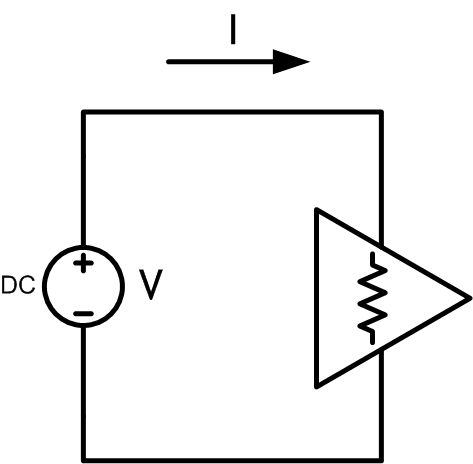
\includegraphics[height=3cm]{leiOhm}
	\caption{Circuito básico com uma fonte de tensão contínua (V) e uma resistência atravessada por uma corrente I.}
	\label{fig:ohm}
\end{figure}

Pode-se calcular a corrente que circula na resistência através da equação \ref{for:ohm}, denominada de Lei de Ohm\index{Lei de Ohm}.

\begin{equation}\label{for:ohm}
	I=\frac{V}{R}
\end{equation}

O texto pode vir em \textbf{negrito} ou em \textit{itálico} ou \textbf{\textit{ambos}}.

O algoritmo \ref{alg1} serve de base para o nosso sistema de controlo do semáforo da igreja.
\begin{algorithm}
\caption{Pseudocódigo para o semáforo}
\label{alg1}
\begin{algorithmic}[1]
\STATE Início
\FOR{todas as luzes}
\IF{sem corrente}
\STATE informar de avaria
\ELSE
\STATE luz ok\ENDIF \ENDFOR
\LOOP
\STATE accionar verde no semáforo principal
\STATE aguardar por sinal dos sensores de posição
\IF{carro no sensor}
\STATE mudar para vermelho semáforo principal
\ENDIF
\ENDLOOP
\STATE \textbf{until} interruptor de manutenção activado
\end{algorithmic}
\end{algorithm}









%% Fim da inserção dos capitulos


%% Inicio Bibliografia
\cleardoublepage
\phantomsection
\addcontentsline{toc}{chapter}{Bibliografia}
%%%%%%%%%%%%%%%%
% Escolher entre as duas opcções
%
% A primeira é a aconselhada pelo despacho reitoral
% A segunda é a utilizada pelo IEEE
%
%Primeira opcção
\bibliographystyle{IEEEtran}				%Estilo bibliografia com nomes
\bibliography{bibliografia}					%Entrada biblbiografia aconselhada com nomes
%
% Segunda opcção
%\bibliographystyle{IEEEtran}					%Estilo bibliografia IEEE
%\bibliography{IEEEabrv,bibliografia}				%Entrada bibliografia aconselhada para IEEE
%% Fim Bibliografia


%%Anexos
\appendix
 
\include{Anexos}
\cleardoublepage


%%Glossário
\newpage
\section*{\titulos{Glossário}}
\vspace{0.5cm}
	\noindent\begin{tabularx}{\linewidth}{l p{0.5cm} Y}
	\LaTeX & & Conjunto de macros para o processador de textos \TeX, utilizado amplamente para a produção de textos matemáticos e científicos devido à sua alta qualidade tipográfica.\cr
	\end{tabularx}
\cleardoublepage



%%Inserir índice remissivo
\printindex

\end{document}
